% Drawing 29/10-2 -- folder 29, batch 10, archive page 183 (PDF page 184).
% Transcription: à droite de « $S \leftarrow S'$ », une esquisse simpliciale : un triangle de sommet $a$ en bas, dont les trois côtés sont fléchés et marqués $d_1$ (à gauche), $d_2$ (en haut) et $d_0$ (à droite), l'intérieur hachuré ; un faisceau de longues flèches le relie à un point $x$ en bas à gauche.
% Kind: simplicial sketch: a triangle with faces d_0, d_1, d_2 and arrows from a point x. Method 2 (schematic redraw from the facsimile). Status: ok.
% Notes: The triangle: the side from a up to the upper left vertex (arrow, marked d_1), the top side as an arrow pointing left towards that vertex (marked d_2), the side from a up to the right vertex (arrow, marked d_0), drawn between the same three vertices, with a few hatching strokes inside; the point a with its letter; the point x at the lower left with its letter; and the bundle of long arrows between x and the triangle: two from x up to the middle of the sheet (heads at the top), one coming down to x from the same place, two from the right vertex down to x, and a double one from x to a. Left out: the long thin line that crosses the sheet obliquely (a separator), a blotted letter above the upper left vertex and a letter above the right vertex (b, uncertain), other sketches of the sheet that enter the crop. Still differs: the arrows of the bundle overlap and their number and direction are a reading; the hatching is free. Overlaid 2026-11-12 (Opus 5.5) on the 400 dpi colour crop and corrected: the two long arrows from the right vertex down towards x ended 6 units short of their heads (now at (22.4, -67.3) and (23.5, -71.7)); the arrows of the upper bundle and of the double arrow x to a, the side d_0 and the point a moved by 1 to 3 units onto the page. Still differs: whether the first of the two long arrows from the right vertex has a head at its lower end is not clear (drawn with one). Redrawn 2026-11-12 (issue 128): to check again. 2026-11-13, Claude Opus 5.5, overlay check (issue 147): every stroke re-read on millimetre grids of the scan rendered at 350 dpi in colour (17-33 px a unit); not compiled (no TeX engine in the session), the TikZ was rasterised by a script and laid over the crop; every stroke, point and label now lies on its ink to within about 1 unit. Changed: the hatching moved 3 to 5 units onto its four strokes, with the small zigzag inside the triangle; the sides d_0 and d_2 and the labels a and d_1 moved by 1 to 2 units. The upper bundle re-read at 30 px a unit: it is two long lines, not three, which overlap over their middle: a thin line from near x up to the middle of the sheet, and a heavy line coming down to x with a heavy head; at the top of the heavy line a heavy hook and a short thin stroke stand on either side of it (together they may be a head pointing up) and are drawn as they are. Of the two long lines from the right vertex, the first starts in a heavy blot and ends near x with no head (the scan settles the earlier doubt); the second ends in a heavy head. The point x is the letter x written heavily, followed by a dot; both are drawn. Left out as before: the separator line, the blotted letter above the upper left vertex, the letter above the right vertex (b, uncertain), the other sketches of the sheet.
% Coordinates: 1 unit = 1 mm = 1/100 of the crop width (bbox in page fractions: [0.59, 0.3, 0.83, 0.455]).
% Redrawn by Claude (claude-fable-5-2), issue #128, 2026-11-12; not checked by a human; not compiled (no TeX in the session).
% Overlaid by Claude (claude-opus-5-5) 2026-11-12 (issue #128): rasterised from its own coordinates over the 400 dpi colour facsimile and corrected from it. Not compiled. Status: partial.
% Rights: reproduces part of the work -- behind RENDER_TRANSCRIPTS, never published by itself.
\documentclass[tikz,border=3pt]{standalone}
\usepackage{amsmath,amssymb}
\usetikzlibrary{patterns,arrows.meta}
\tikzset{pencil/.style={black!45}, struck/.style={black!35}, mpt/.style={circle,draw,inner sep=1.3pt}, pt/.style={circle,fill,inner sep=0.9pt}, opt/.style={circle,draw,fill=white,inner sep=1.1pt}}
\begin{document}
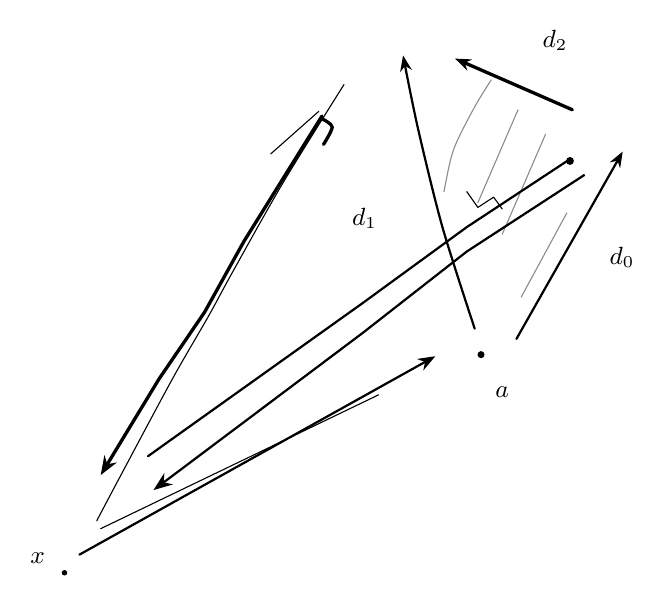
\begin{tikzpicture}[x=1mm,y=1mm,line cap=round,line join=round,font=\scriptsize]
% the triangle: d_1 from a up to the upper left vertex, d_2 along the top towards it, d_0 from a up to the right vertex
\draw[thick,-{Stealth[length=2mm]}] plot[smooth] coordinates {(64.3,-51.6) (60.2,-38.7) (57.1,-26.2) (55.2,-16.9)};
\draw[very thick,-{Stealth[length=2mm]}] (76.7,-23.8) -- (61.8,-17.3);
\draw[thick,-{Stealth[length=2mm]}] (69.6,-52.9) -- (83.1,-29.1);
% hatching strokes and a small zigzag inside
\draw[pencil] plot[smooth] coordinates {(60.4,-34.2) (61.6,-28.9) (64.2,-23.6) (66.4,-20)};
\draw[pencil] (64.7,-35.6) -- (69.8,-23.8);
\draw[pencil] (67.8,-39.6) -- (73.3,-26.9);
\draw[pencil] (70.2,-47.6) -- (76,-36.9);
\draw (63.3,-34.2) -- (64.7,-36.2) -- (66.7,-34.9) -- (67.8,-36.4);
\node[pt] at (65.1,-54.9) {};
\node[inner sep=1pt] at (67.8,-59.6) {\small $a$};
% the point x (the letter written heavily, a dot after it)
\node[inner sep=1pt] at (8.8,-80.7) {\small $x$};
\fill (12.2,-82.6) circle[radius=0.35];
% the upper bundle: a thin line from near x up to the middle of the sheet, and a heavy line coming down to x with a heavy head; they overlap over their middle
\draw plot[smooth] coordinates {(16.3,-76) (19.1,-70.7) (25.9,-58) (30.5,-50) (33.5,-44.5) (40,-33) (47.7,-20.6)};
\draw[very thick,-{Stealth[length=2.4mm]}] (44.9,-24.6) -- (35,-40.5) -- (30,-49.5) -- (24.2,-58) -- (16.8,-70.2);
% at the top of the heavy line: a heavy hook and a short thin stroke (together they may be a head pointing up)
\draw[very thick] plot[smooth] coordinates {(45,-25) (46.2,-26) (45.1,-28.2)};
\draw (38.4,-29.4) -- (44.5,-24);
% from the right vertex down to x: a line with a heavy end at the top and no head, and an arrow
\fill (76.4,-30.3) circle[radius=0.5];
\draw[thick] (76.2,-30.2) -- (63.3,-38.7) -- (50,-48.4) -- (22.8,-67.8);
\draw[thick,-{Stealth[length=2.4mm]}] (78.2,-32.1) -- (63.3,-41.8) -- (50,-52.2) -- (23.5,-72.1);
% the double arrow from x to a
\draw[thick,-{Stealth[length=2.2mm]}] (14.1,-80.3) -- (59.3,-55.1);
\draw (16.8,-77) -- (52.1,-60);
\node[inner sep=1pt] at (50.3,-37.6) {\small $d_1$};
\node[inner sep=1pt] at (74.5,-15) {\small $d_2$};
\node[inner sep=1pt] at (83,-42.5) {\small $d_0$};
\end{tikzpicture}
\end{document}
